\documentclass{article}

\usepackage{graphicx}
\usepackage{tikz}
\usepackage{tikzsymbols}
\usetikzlibrary{calc,patterns,shapes.geometric}
\pagestyle{empty}
\usepackage[margin=0pt]{geometry}
\geometry{papersize={14in,12in}}

\def\centerarc[#1](#2)(#3:#4:#5){\draw[#1] ($(#2)+({#5*cos(#3)},{#5*sin(#3)})$) arc (#3:#4:#5);}

\begin{document}
	\begin{figure}
		\centering
		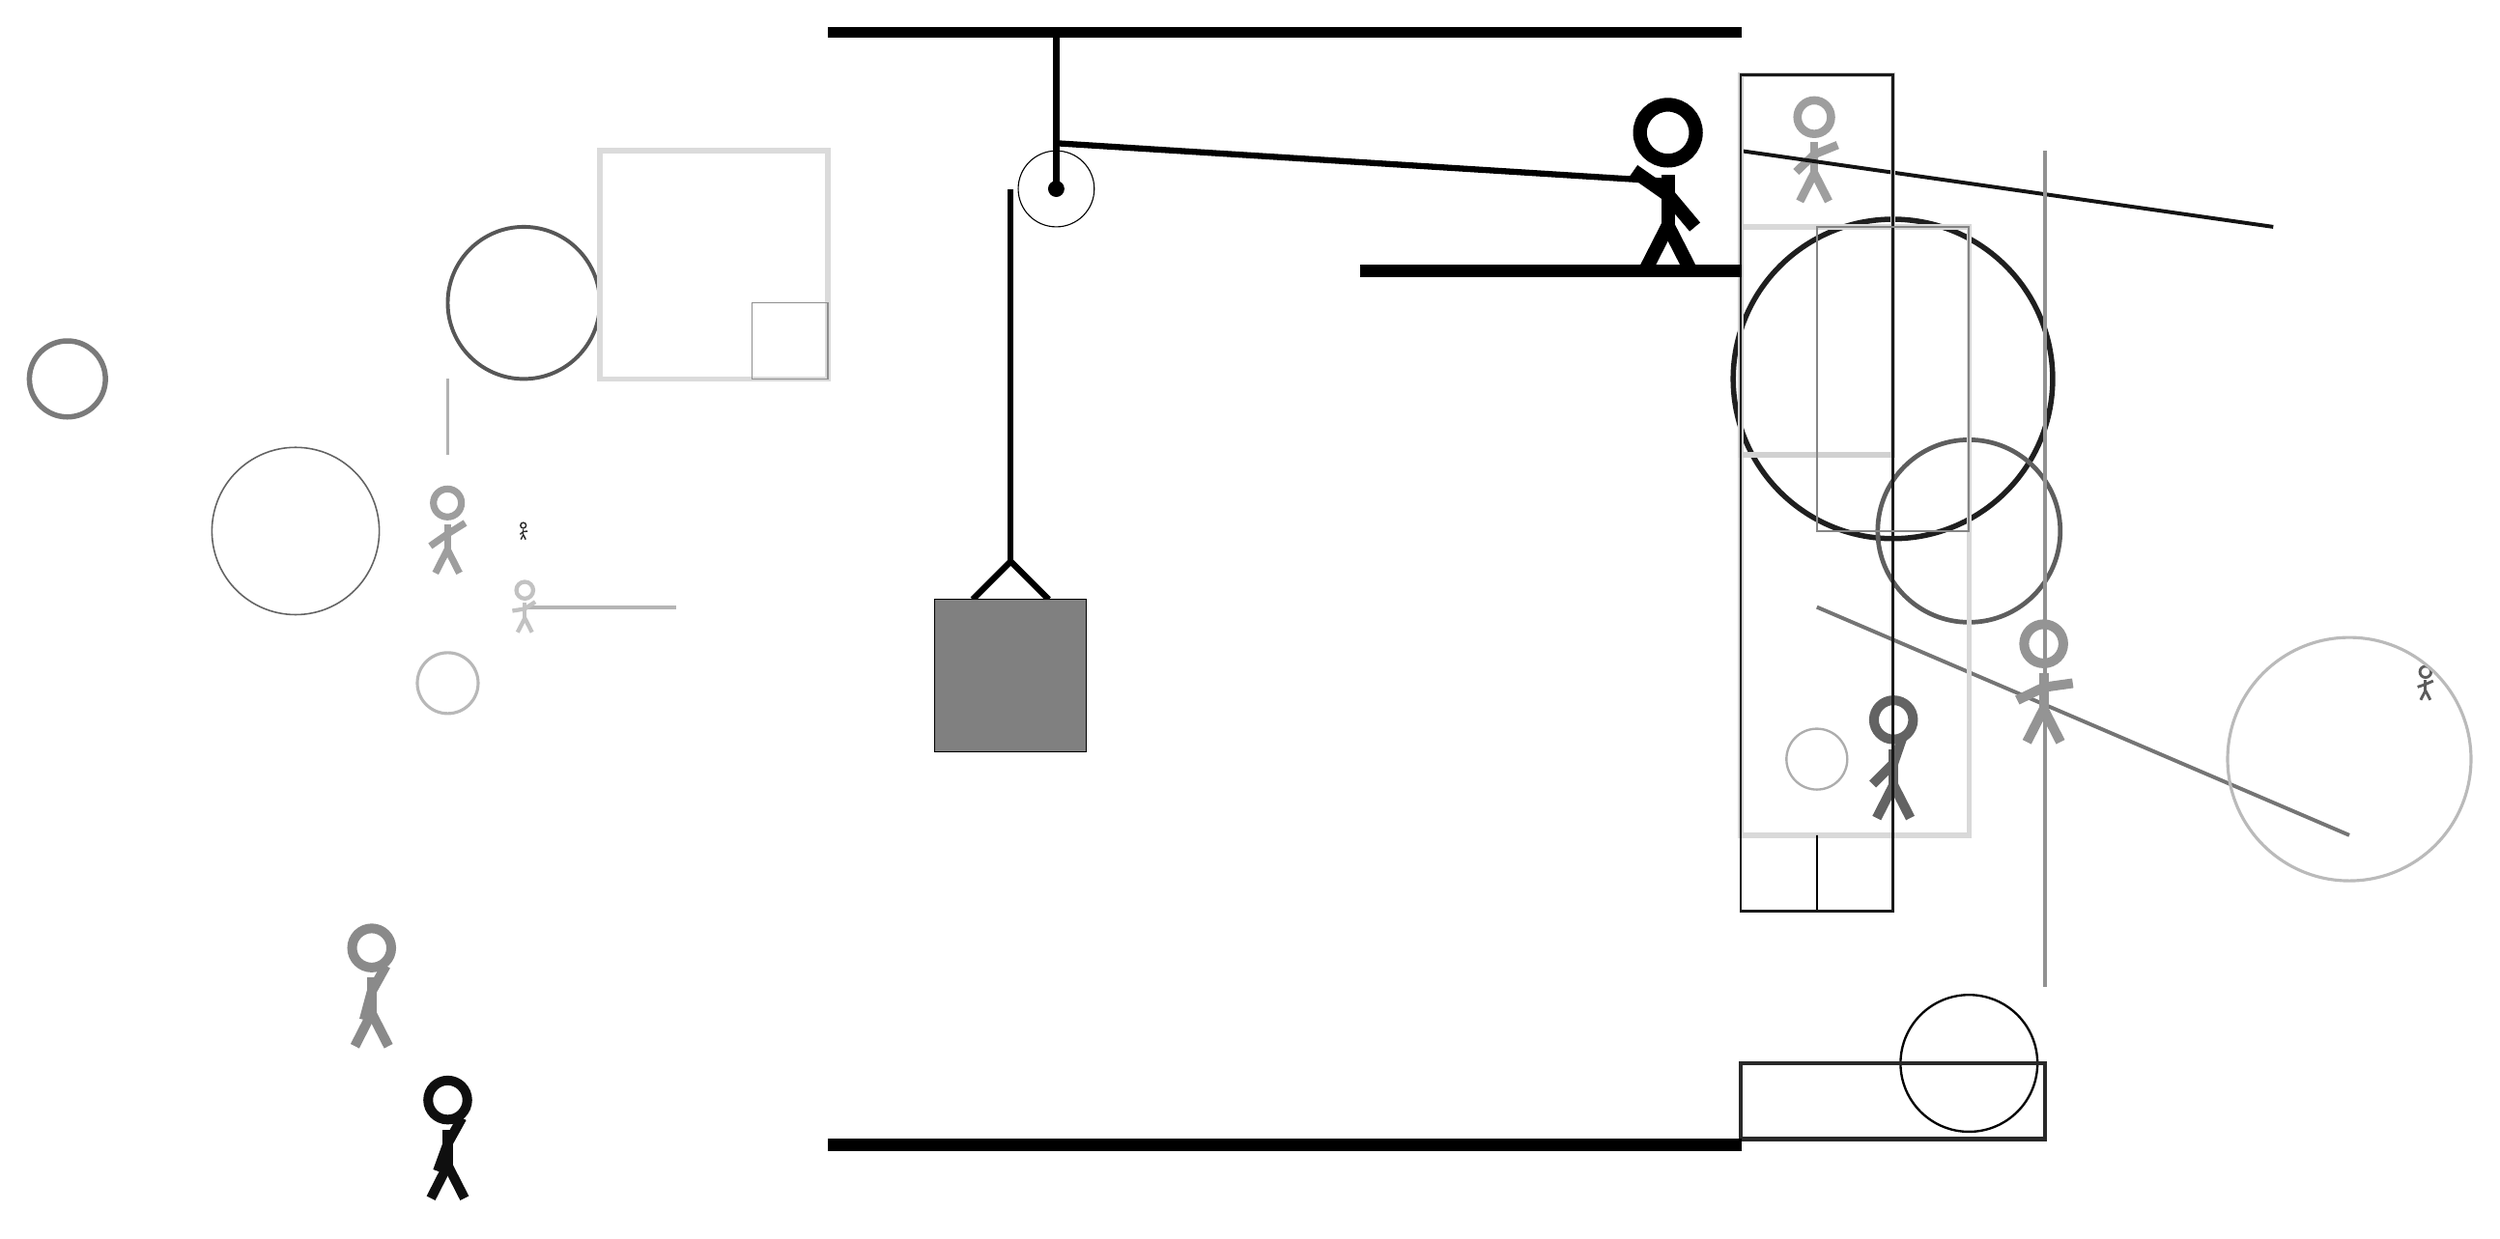
\begin{tikzpicture}
			%%%%% START %%%%%
			
			\draw[fill=black] (-2, 11.5) rectangle (10, 11.625);
			
			\draw (1, 9.5) circle (0.5);
			\draw[fill=black] (1, 9.5) circle (0.1);
			\draw[line width=0.8mm] (1, 11.5) -- (1, 9.5);
			
			\draw[line width=0.8mm](-0.1, 4.1) --  (0.4, 4.6) -- (0.9, 4.1);
			\draw[fill=black!50] (-0.6, 4.1) rectangle (1.4, 2.1);
			
			\draw [line width=0.7mm, color=black!88](12, 7) circle (2.1);
			
			\node[line width=0.3mm, color=black!61] at (12, 2) {\Strichmaxerl[7][45][71]};
			\draw[line width=0.5mm, color=black!54](11, 4) -- (18, 1);
			\draw [line width=0.6mm, color=black!63](13, 5) circle (1.2);
			
			\draw [line width=0.2mm, color=black!61](-9, 5) circle (1.1);
			
			\draw [line width=0.4mm, color=black!28](-7, 3) circle (0.4);
			
			\node[line width=0.6mm, color=black!64] at (19, 3) {\Strichmaxerl[2][19][24]};
			\draw [line width=0.5mm, color=black!66](-6, 8) circle (1.0);
			\draw[line width=0.5mm, color=black!29](-4, 4) -- (-6, 4);
			\node[line width=0.6mm, color=black!38] at (11, 10) {\Strichmaxerl[6][44][22]};
			\draw [line width=0.3mm, color=black!98](13, -2) circle (0.9);
			
			\draw[line width=0.7mm, color=black!15] (10, 1) rectangle (13, 9);
			\draw[line width=0.5mm, color=black!92](10, 10) -- (17, 9);
			
			\draw[line width=0.6mm, color=black!84] (10, -2) rectangle (14, -3);
			\draw[line width=0.5mm, color=black!43](14, 10) -- (14, -1);
			\draw[line width=0.3mm, color=black!100] (11, 0) rectangle (11, 1);
			
			\node[line width=0.5mm, color=black!94] at (-7, -3) {\Strichmaxerl[7][70][61]};
			
			\node[line width=0.6mm, color=black!42] at (14, 3) {\Strichmaxerl[7][26][8]};
			\draw [line width=0.4mm, color=black!27](18, 2) circle (1.6);
			\draw[line width=0.7mm, color=black!18] (10, 6) rectangle (12, 11);
			\draw [line width=0.3mm, color=black!32](11, 2) circle (0.4);
			
			\node[line width=0.4mm, color=black!24] at (-6, 4) {\Strichmaxerl[3][9][34]};
			\draw[line width=0.7mm, color=black!14] (-2, 10) rectangle (-5, 7);
			\node[line width=0.2mm, color=black!46] at (-8, -1) {\Strichmaxerl[7][75][61]};
			\node[line width=0.4mm, color=black!84] at (-6, 5) {\Strichmaxerl[1][41][6]};
			
			\draw[line width=0.3mm, color=black!90] (12, 11) rectangle (10, 0);
			\node[line width=0.2mm, color=black!38] at (-7, 5) {\Strichmaxerl[5][35][32]};
			\draw [line width=0.7mm, color=black!52](-12, 7) circle (0.5);
			
			\draw[line width=0.2mm, color=black!44] (-2, 8) rectangle (-3, 7);
			\draw[line width=0.3mm, color=black!48] (11, 9) rectangle (13, 5);
			\draw[line width=0.5mm, color=black!30](-7, 7) -- (-7, 6);
			
			
			\draw[line width=0.8mm](0.4, 9.5) -- (0.4, 4.6);
			\centerarc[line width=0.8mm](1, 9.5)(90:180:0.6)
			\draw[line width=0.8mm](1, 10.1) -- (9, 9.6);
			
			\node at (9, 9.5) {\Strichmaxerl[10][-35][-50]};
			\draw[fill=black] (5, 8.5) rectangle (10, 8.35);
			
			\draw[fill=black] (-2, -3) rectangle (10, -3.15);
			
			%%%%% END %%%%%
		\end{tikzpicture}
	\end{figure}	
\end{document}